% BANKS-SOURCE: pdf=50 print=40 kind=section id=4.3
\subsection{Field theory for massive spin-1 particles}

% BANKS-SOURCE: pdf=50 print=40 kind=prose
The analysis we did of the states of massive spinning particles implies that the creation
operators of massive spin-1 particles satisfy

% BANKS-SOURCE: pdf=50 print=40 kind=display id=4.3a
\begin{equation*}
  U(\Lambda)a_i^\dagger(\mathbf p)U^{-1}(\Lambda)
  =\sqrt{\frac{\omega_{\boldsymbol{\Lambda p}}}{\omega_{\mathbf p}}}\,
  R_i{}^j(W(\Lambda,p))a_j^\dagger(\boldsymbol{\Lambda p}),
\end{equation*}
where $R$ is the usual $(D-1)\times(D-1)$ matrix representation of rotations,
three-dimensional in $D=4$.

For the $D$-dimensional massive vector, the spatial indices run over
$i,j=1,\ldots,D-1$ and $R$ is the vector representation of $\mathrm{SO}(D-1)$;
the displayed three-dimensional statement is its $D=4$ specialization.

% BANKS-SOURCE: pdf=50 print=40 kind=prose
As in the scalar case we want to find a local field linear in creation and annihilation
operators, which is a model for a device that can create maximally localized states of a
single particle. The covariant field we construct from the creation operators must have at
least $D-1$ components, each of which transforms as a vector under rotations. The
stability subgroup of a single space-time point, in the Poincaré group, is the Lorentz
group, so the fields at a point should transform as a representation of this group. The
particle momentum is Fourier conjugate to its position, so the components of the field
are related to internal degrees of freedom of the particle. We have described particles
with a finite number of degrees of freedom per momentum state, so we should have
fields that transform in finite-dimensional representations of the Lorentz group. None
of these representations is unitary, but we are not talking about the action of the Lorentz
group on the Hilbert space. If that unitary action is denoted $U(\Lambda)$ then we want the
field $A_K$ to transform as

% BANKS-SOURCE: pdf=50 print=40 kind=display id=4.3b
\begin{equation*}
  U(\Lambda)A_K(x)U^{-1}(\Lambda)=S_K{}^L(\Lambda^{-1})A_L(\Lambda x),
\end{equation*}
where $S(\Lambda)$ is the finite-dimensional representation. $S$ is not a unitary matrix, but
$U(\Lambda)$ is an infinite-dimensional unitary operator, which we constructed in the previous
section.

% BANKS-SOURCE: pdf=50 print=40 kind=prose
In $D=4$, the only three-dimensional representations of the Lorentz group are the (complex)
self-dual and anti-self-dual tensors
\begin{equation*}
  B_{\mu\nu}=\pm\frac{\ii}{2}\epsilon_{\mu\nu\rho\sigma}B^{\rho\sigma}.
\end{equation*}
where $\epsilon^{0123}=+1$ and the factor of $\ii$ reflects $*^2=-1$ on Lorentzian
two-forms. These are mapped into each other by reflection. In order to construct a Hermitian
Hamiltonian we would need both of these fields, so we really have six real components.
The smallest representation we can use to describe spin-1 particles is the $D$-vector $B_\mu$,
and this can be reduced to $D-1$ components, three in $D=4$, by the covariant constraint
\begin{equation*}
  \partial_\mu B^\mu=0.
\end{equation*}

% BANKS-SOURCE: pdf=51 print=41 kind=prose
Thus we may guess at a formula
\begin{equation*}
  B_\mu(x)=\int\frac{\dd^{D-1}\mathbf p}
  {\sqrt{2\omega_{\mathbf p}(2\pi)^{D-1}}}
  \left[\epsilon_\mu{}^i(p)a_i(\mathbf p)\ee^{+\ii p\cdot x}
  +\mathrm{h.c.}\right],
\end{equation*}
where $p^\mu\epsilon_\mu(p)=0$.
There are $D-1$ solutions to the latter equation, three in $D=4$. We normalize the spatial component
of $\epsilon_\mu$ by $\epsilon_i{}^j(\mathbf p=\mathbf0)=\delta_i^j$, and allow it to transform as a $D$-vector, which defines it for all
values of $p$. In the exercises, the reader will verify that this choice leads to a Lorentz
$D$-vector transformation law for the field $B_\mu(x)$. We can build an anti-symmetric tensor
\begin{equation*}
  B_{\mu\nu}=\partial_\nu B_\mu-\partial_\mu B_\nu,
\end{equation*}
so we see that the $D(D-1)/2$-component anti-symmetric tensor is a derived field, six in $D=4$. Since $B_\mu$ was
constructed to satisfy the Klein--Gordon equation and the transversality condition
$\partial_\mu B^\mu=0$, this field satisfies
\begin{equation*}
  \partial_\nu B^{\mu\nu}-\mu^2B^\mu=0,
\end{equation*}
which is called the Proca \cite{banks-ref-24} equation. Note that, conversely, the Proca equation implies
the transversality condition.

% BANKS-SOURCE: pdf=51 print=41 kind=display id=4.3c
A Lagrangian that leads to the Proca equation is
\begin{equation*}
  \mathcal{L}_P=-\frac14B_{\mu\nu}B^{\mu\nu}-\frac{\mu^2}{2}B_\mu B^\mu.
\end{equation*}
To canonically quantize this Lagrangian (see the problems) we must use the constraint
equation to eliminate $B_0$, which does not have a canonical conjugate. The procedure is
slightly painful, but ends up giving the obvious answer: the generating functional for
Green functions $Z[J^\mu]$ is given by a functional integral with this Lagrangian coupled to
a source via $\delta\mathcal{L}=B_\mu J^\mu$. The generating functional for free connected Green functions
is obtained by doing a Gaussian integral:
\begin{equation*}
  W_0[J^\mu]=\frac{1}{2}\int\dd^D x\,\dd^D y\,J^\mu(x)J^\nu(y)
  \int\frac{\dd^D p}{(2\pi)^D}\ee^{+\ii p\cdot(x-y)}
  \frac{\eta_{\mu\nu}+p_\mu p_\nu/\mu^2}{p^2+\mu^2-\ii\epsilon}.
\end{equation*}
The reader should be able to see from this expression’s symmetry that it would be
inconsistent to quantize these fields as fermions. As in the case of spin-zero particles,
the connected two-point function of the free Proca field is just the Green function
(in the sense of partial differential equations) of the Proca equation, with Feynman
boundary conditions.

\BanksImplicitHook{I-CH04-001}

It should by now be obvious how to derive Feynman diagrams for any perturbation
around this free-field Lagrangian. It would be a good idea for the reader to work out
the diagrams for two-, three- and four-point functions up to one loop (without doing
the loop integrals) for the interaction
$\mathcal{L}_I=\ii gB_\mu(\phi^*\partial^\mu\phi-\phi\,\partial^\mu\phi^*)$
between the Proca field and a charged scalar.

% BANKS-SOURCE: pdf=52 print=42 kind=prose
The propagator of a massive vector boson\footnote[3]{Here and henceforth, we record the Feynman rules in both Minkowski and Euclidean space.}
will be denoted by

% BANKS-SOURCE: pdf=52 print=42 kind=figure id=unnumbered-main-ch4-massive-photon-propagator
\begin{center}
\resizebox{\linewidth}{!}{%
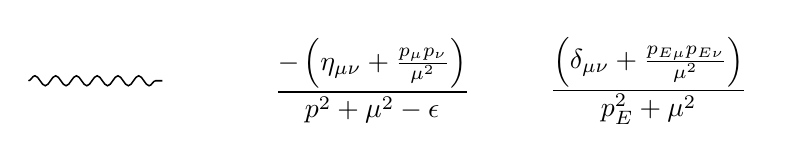
\begin{tikzpicture}[x=1cm,y=1cm,baseline=(current bounding box.center)]
  \draw[line width=.55pt,decorate,
        decoration={snake,amplitude=1.8pt,segment length=7.5pt}] (0,0) -- (1.7,0);
  \node[anchor=west] at (3.0,0) {$\displaystyle
    \frac{-\ii\left(\eta_{\mu\nu}+\frac{p_\mu p_\nu}{\mu^2}\right)}{p^2+\mu^2-\ii\epsilon}$};
  \node[anchor=west] at (6.5,0) {$\displaystyle
    \frac{\left(\delta_{\mu\nu}+\frac{p_{E\mu}p_{E\nu}}{\mu^2}\right)}{p_E^2+\mu^2}$};
\end{tikzpicture}%
}

\end{center}
\BanksSourceNote{Massive photon propagator in Minkowski and Euclidean signature}

\BanksImplicitHook{I-CH04-002}
\BanksImplicitHook{I-CH04-003}

% BANKS-SOURCE: pdf=52 print=42 kind=prose
One look at the vector boson propagator tells us that something dramatic happens
for spin 1 and zero mass. Indeed, the longitudinal part of the propagator blows up in
this limit. The only way we can get a consistent limiting expression is to insist that the
source satisfy $\partial_\mu J^\mu=0$. A massless vector meson must be coupled to a conserved current.
This remark becomes even more interesting when we realize that the $\mu=0$ limit of the
Proca equation coupled to a source is just Maxwell’s equation for the electromagnetic
field.

% BANKS-SOURCE: pdf=52 print=42 kind=subsection id=4.3.1
\subsubsection{The Stueckelberg formalism}

% BANKS-SOURCE: pdf=52 print=42 kind=prose
We can obtain more insight by introducing a redundant parametrization of the space
of field variables, known as the Stueckelberg formalism. We introduce another vector
field $A_\mu$, as well as a scalar, $\theta$, via the formula
\begin{equation*}
  B_\mu=A_\mu-\partial_\mu\theta.
\end{equation*}
The Lagrangian is obtained by just substituting this combination into the Proca
Lagrangian. The well-known gauge invariance of Maxwell’s field strength tensor with
respect to gauge transformations of the vector potential implies that
\begin{equation*}
  B_{\mu\nu}=\partial_\nu A_\mu-\partial_\mu A_\nu\equiv F_{\mu\nu}.
\end{equation*}
The full Lagrangian now has a gauge invariance under
\begin{equation*}
  A_\mu\longrightarrow A_\mu+\partial_\mu\Omega,
  \qquad \theta\longrightarrow\theta+\Omega,
\end{equation*}
even for non-zero mass. If we couple a current to $A_\mu$, then it must be conserved, in order
to preserve gauge invariance (one must integrate by parts to show this, which means
that either the gauge transformation or the current must vanish sufficiently rapidly at
infinity). If it is conserved, then $\int J^\mu A_\mu=\int J^\mu B_\mu$. For such conserved sources, the
longitudinal part of the $B_\mu$ propagator cancels out, and there are no divergences when
$\mu\to0$.

\BanksImplicitHook{I-CH04-004}

% BANKS-SOURCE: pdf=52 print=42 kind=prose
From the point of view of free-particle physics, Maxwell’s gauge invariance is thus
the result of the discontinuity of the number of degrees of freedom of a spin-1 particle

% BANKS-SOURCE: pdf=53 print=43 kind=prose
in the massless limit. The Stueckelberg formalism incorporates the massless split of the
degrees of freedom into a spin-zero particle and a massless helicity $\pm1$ particle into
the massive theory by introducing a redundant degree of freedom. It is a hint of the Higgs
mechanism, which we will discuss in Chapters 6 and 8. The connection between gauge
invariance and a redundancy of degrees of freedom will reappear again and again in
our discussions.
